\documentclass{jsarticle}
\usepackage[dvipdfmx]{graphicx}
\usepackage{bm}
\usepackage{amsmath}
\usepackage{amssymb}
\usepackage{amsfonts}
\usepackage{comment}
\usepackage{listings}
\usepackage{cases}
\lstset{
    basicstyle={\ttfamily},
    identifierstyle={\small},
    commentstyle={\smallitshape},
    keywordstyle={\small\bfseries},
    ndkeywordstyle={\small},
    stringstyle={\small\ttfamily},
    frame={tb},
    breaklines=true,
    columns=[l]{fullflexible},
    numbers=left,
    xrightmargin=0zw,
    xleftmargin=3zw,
    numberstyle={\scriptsize},
    stepnumber=1,
    numbersep=1zw,
    lineskip=-0.5ex,
    keepspaces=true,
    language=c
}
\renewcommand{\lstlistingname}{リスト}
\makeatletter
\newcommand{\figcaption}[1]{\def\@captype{figure}\caption{#1}}
\newcommand{\tblcaption}[1]{\def\@captype{table}\caption{#1}}
\makeatother

\title{科学技術英語 英文読解課題}
\author{Ec5 24番 平田 蓮}
\date{}

\begin{document}
\maketitle
\section*{付録A 発展的なNumPy}
    この付録では、配列計算のためのNumPyライブラリをより深く掘り下げていきます。
    これにはndarray型の内部の詳細や、より高度な配列操作とそのアルゴリズムが含まれます。

    この付録は雑多な内容を含んでおり続けて読む必要はありません。

    \subsection*{A.1 ndarrayオブジェクトの内部構造}
        NumPyのndarrayは、同じ型のデータのブロックを
        (連続か区切られているかにかかわらず)
        多次元配列オブジェクトとして提供します。
        データ型(dtype)は、データが浮動小数点、整数、真偽値、
        あるいはこれまで見てきた他の型のどれであるかを決定します。

        ndarrayを柔軟にしている理由の一つに、
        すべての配列オブジェクトがデータをブロック区切りでみていることがあります。
        例えば配列に対する参照\verb|arr[::2, ::-1]|がデータを一切コピー
        していないことを不思議に思うかもしれません。
        その理由は、ndarrayは単なるデータとその型の集まりではなく、
        配列がメモリ内をさまざまなステップサイズで移動できるようにする「ストライド」
        情報を持っているからです。
        より正確に言うと、ndarrayの内部は以下のような構成になっています。

        \begin{itemize}
            \item RAMやメモリマップ内にあるデータの集まりへのポインタ
            \item 配列内の一定個数のデータの型
            \item 配列の形を表すタプル
            \item 各次元に沿って要素を一つ進めるために遷移するバイト数(整数値)のタプル
        \end{itemize}

        図\ref{fig:A-1}は、ndarrayの内部構造を示す模式図です。

        \begin{figure}[h]
            \centering
            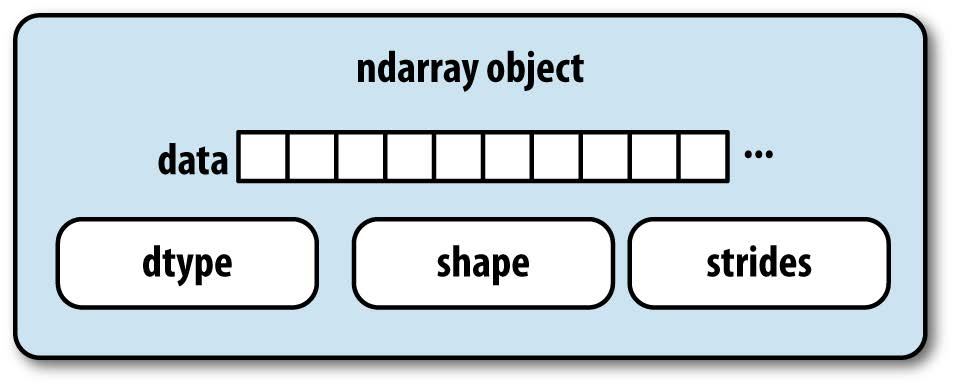
\includegraphics[width=10cm]{images/A-1.jpg}
            \caption{NumPyのndarrayオブジェクト}
            \label{fig:A-1}
        \end{figure}

        例えば、10 $\times$ 5の配列は\verb|(10, 5)|の形を持っています。

        \begin{lstlisting}
np.ones((10, 5)).shape # (10, 5)\end{lstlisting}

        float64(8バイト)型の典型的な3$\times$4$\times$5配列は、
        \verb|(160, 40, 8)|のストライドを持っています。
        (一般的に特定の軸のストライドが大きいほど、
        その軸に沿って計算を行うコストが高くなるので、
        ストライドについて知っておくと便利です。)

        \begin{lstlisting}
np.ones((3, 4, 5), dtype=np.float64).strides # (160, 40, 8)\end{lstlisting}

        典型的なNumPyユーザーが配列のストライドに興味を持つことは稀ですが、
        ストライドは0配列をコピー、構築するための重要な要素です。
        ストライドには負の値を設定することもでき、
        配列をメモリ上で逆向きに移動させることができます
        (例えば、\verb|obj[::-1]|や\verb|obj[:, ::-1]|
        のようなスライスがこれに該当します)。
\end{document}